Experimental Results (recommended size: 1.5 pages)

\begin{enumerate}[(a)]
	\item Experimental setup: describe the working environments (DAS, Amazon EC2,
	etc.), the general workload and monitoring tools and libraries, other tools and libraries you have used to implement and deploy your system, other tools and libraries used to conduct your experiments.
	\item Experiments: describe the experiments you have conducted to analyze each system feature, then analyze them; use one sub-section per experiment. For each experiment, describe the workload, present the operation of the system, and analyze the results. In the analysis, report:
	\begin{enumerate}
		\item Charged-time = time that would have been charged using the Amazon EC2 timing approach (1-hour increments)
		\item Charged-cost = cost that would have been charged using the 3
		E
		Amazon EC2 charging approach, assuming 10 Euro-cents/charged hour
		\item Service metrics of the experiment, such as runtime and response time of
		the service, etc.
		\item (optional) Usage metrics of the experiment, such as per-VM and overall
		system usage and activity.
	\end{enumerate}
\end{enumerate}

We evaluate the performance of \appName{} by running it on the Amazon EC2 cloud, which provides a web interface through which images for virtual machines can be created, managed, and launched.
We create one image containing our load balancer and one image containing code for the solver machine.
We need to launch only the load balancer image, which will launch solver instances on its own depending on workload.
In the instance overview of the EC2 web interface we can find the IP address of the machines so we can make Sudoku request to the load balancer. 

The workload is generated by a Java program running locally on our own machines.
It contains a large list of partially completed puzzles. Within random intervals the program selects a random puzzle from the list a makes a GET request to the load balancer.   
The workload program is multithreaded to allow new requests to be made while others are still active.
Alongside the workload generation there is a monitoring thread which inspects and logs data from the load balancer such as the number of active machines and resource usage.

Figure~\ref{fig:asdf} shows the workload and the number of solver machines over a period of time. Machines allocated when the workload is high, and they are terminated when it drops. 

\begin{figure}[H]
	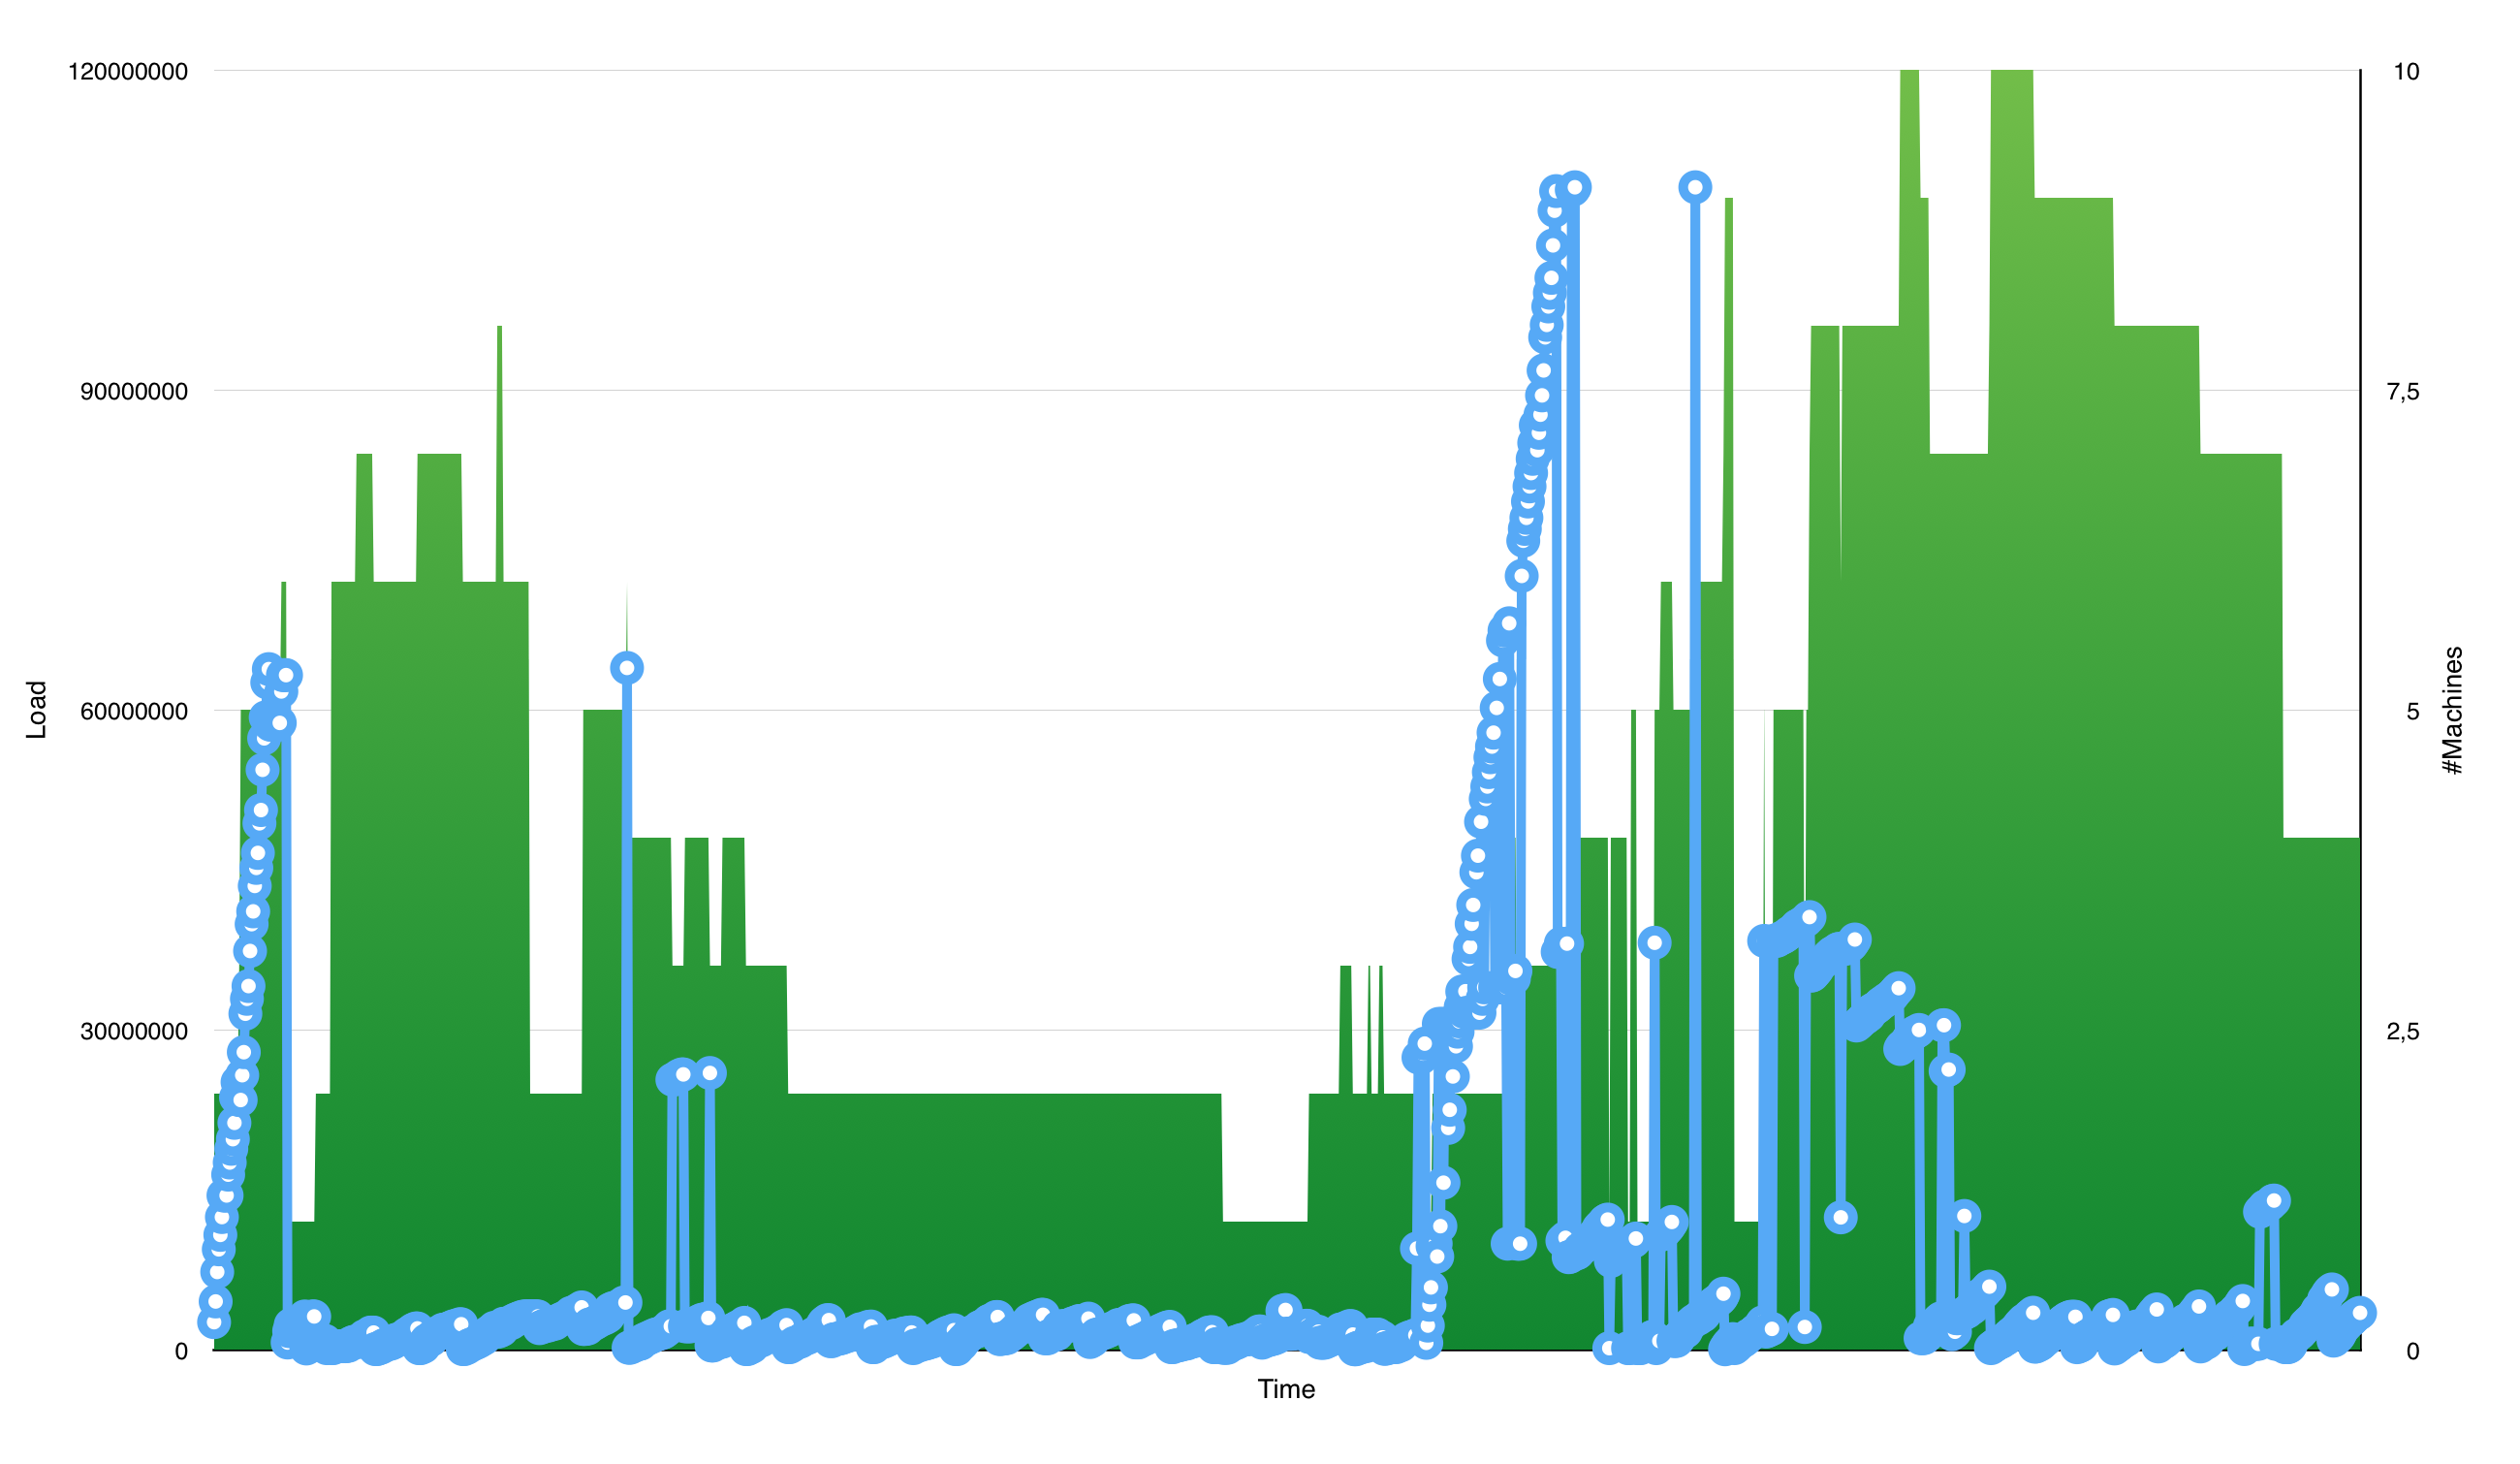
\includegraphics[width=\linewidth]{load_and_machines}
	\caption{The workload(blue) and the number of machines(green) plotted over time}
	\label{fig:asdf}
\end{figure}


Figure~\ref{fig:exp:response} shows the distribution of the response time the end user experiences when making a request. Data for this experiment was gathered during varying workload. It shows that although there is some variation, the delay is always less than 60 milliseconds.

\begin{figure}[H]
	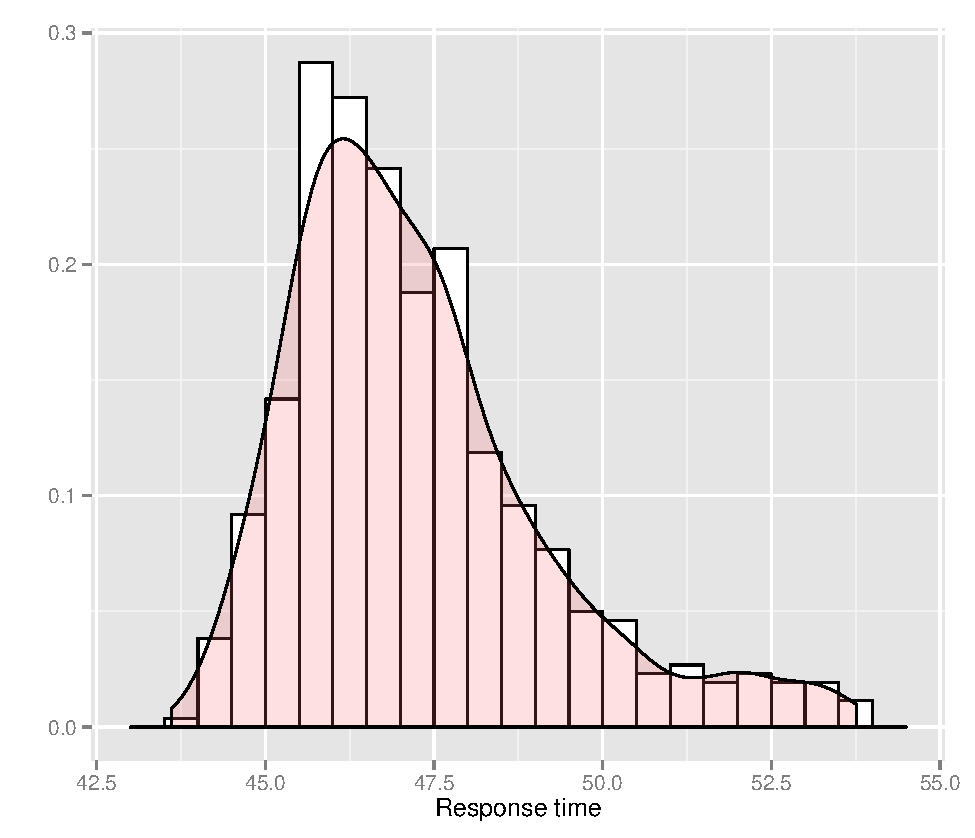
\includegraphics[width=\linewidth]{hist_response_time}
	\caption{Distribution of the response time in milliseconds of the server, with outliers removed}
	\label{fig:exp:response}
\end{figure}
